\subsection{送信波形の計測}
透過波形の計測に先立ち、入射波形に関する情報を得ることを目的として、
ラインフォーカス探触子先端部を供試体に接触させず、自由に振動させたときの
挙動を調べた。振動波形の取得にはLDVを用い、探触子の駆動は前節で述べた
条件によって行った。その結果得られた、探触子先端部の振動波形を図\ref{fig:fig5}に示す。
この図の(a)は振動速度の時刻歴を、(b)はその周波数スペクトルを示している。
時刻歴波形からは、シュー内部を超音波が伝播することによる時間遅れが
約11$\mu$secであることが読み取れる。また振幅値は、peak-to-peakで
およそ0.4V程度であることがわかる。これは、別途行った2.25MHZ、
直径22.5mmの垂直接触型トランスデューサに比べ、約20倍程度大きな
振幅値で、圧電素子からの縦波がシュー先端部に集束し、強い超音波が励起
されていることを裏付けている。また,周波数スペクトルからは、周波数帯域
の上限が約3MHz、主たる周波数成分は1〜2MHにあることがわかる。
なお、シュー先端部で反射された波が、再度先端部に集束することも確認しているが、そ
の波形成分は30$\mu$sec付近にあり、時間軸上で完全に分離でき、以下で示す
計測の障害にはならない。
%--------------------
\begin{figure}[h]
	\begin{center}
	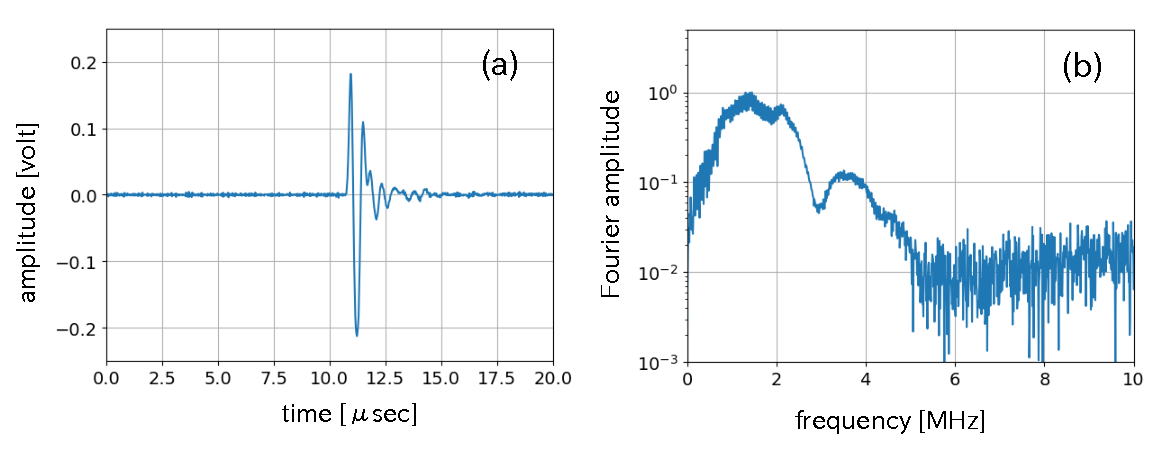
\includegraphics[width=0.9\linewidth]{Figs/fig5.eps} 
	\end{center}
	\caption{
		レーザードップラー振動計で計測したラインフォーカス探触子シュー先端部の振動速度波形.
	} 
	\label{fig:fig5}
\end{figure}
%--------------------
\subsection{透過波波形}
花崗岩コア供試体を用いて計測した、透過波の時刻歴波形を図\ref{fig:fig5_2}と\ref{fig:fig5_3}に示す。
これらの図には、入射方向の異なる6つの走時プロットを示している。
各々の走時プロットは、横軸が時間$t$($\mu$sec)を、縦軸は計測位置の$y$座標(mm)を表し,
$(t,y)$で観測された波形振幅をカラー表示している。
なお、波形振幅は、測線内で観測される最大振幅で無次元化している。
いずれの入射方向でも、19$\mu$sec前後に大きな振幅を持つ、位相の揃った表面波が到達し、その後、
多重散乱に起因したコーダ波が20$\mu$sec程度継続して観測されている。
位相の揃った初動成分の振幅は、場所によって大きな変動があり、波形も計測位置や入射方向に
よって異なることが分かる。このことから、個々の観測波形のピーク位置や到達時間から、
伝播速度を正確に求めることは困難であることが分かる。
そこで以下では、測線上で観測された波形データ全てを使い、平均的な表面波伝播速度を求める。
伝播速度は、群遅延から求めた群速度と、相互相関関数で評価した遅延時間から求めた
音速のに種類を入射方向毎に求め、供試体の音響異方性を調べる。
%--------------------
\begin{figure}[h]
	\begin{center}
	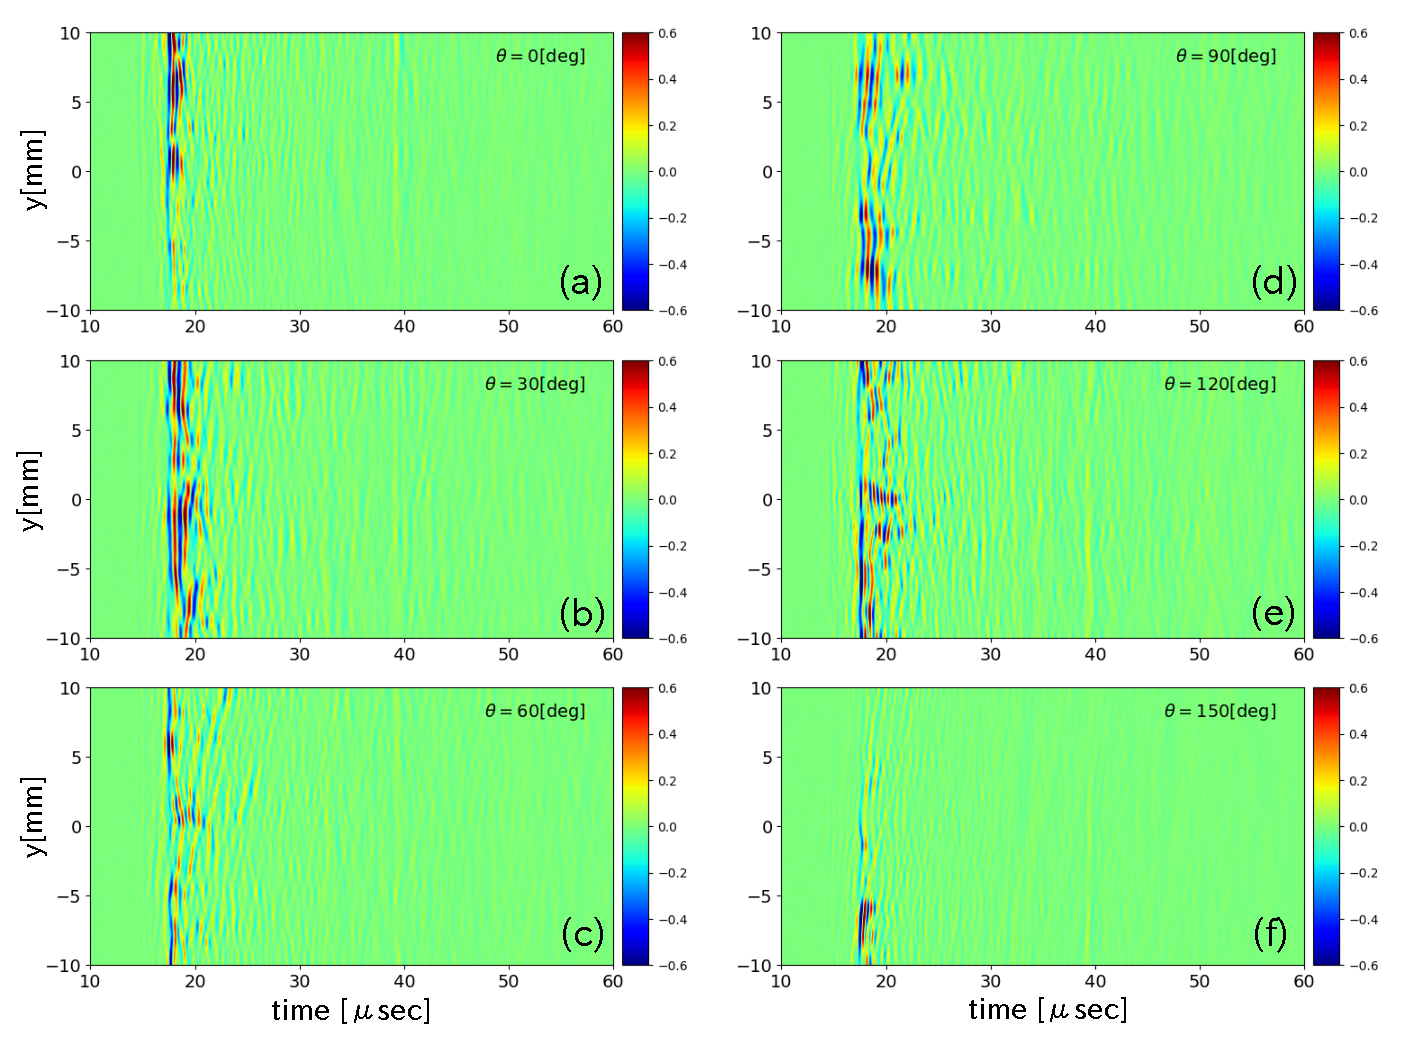
\includegraphics[width=1.0\linewidth]{Figs/fig5_2.eps} 
	\end{center}
	\caption{
		透過波波形の走時プロット(入射方向$\theta=0\sim 150^{\circ}$)
	} 
	\label{fig:fig5_2}
\end{figure}
%--------------------
\begin{figure}[h]
	\begin{center}
	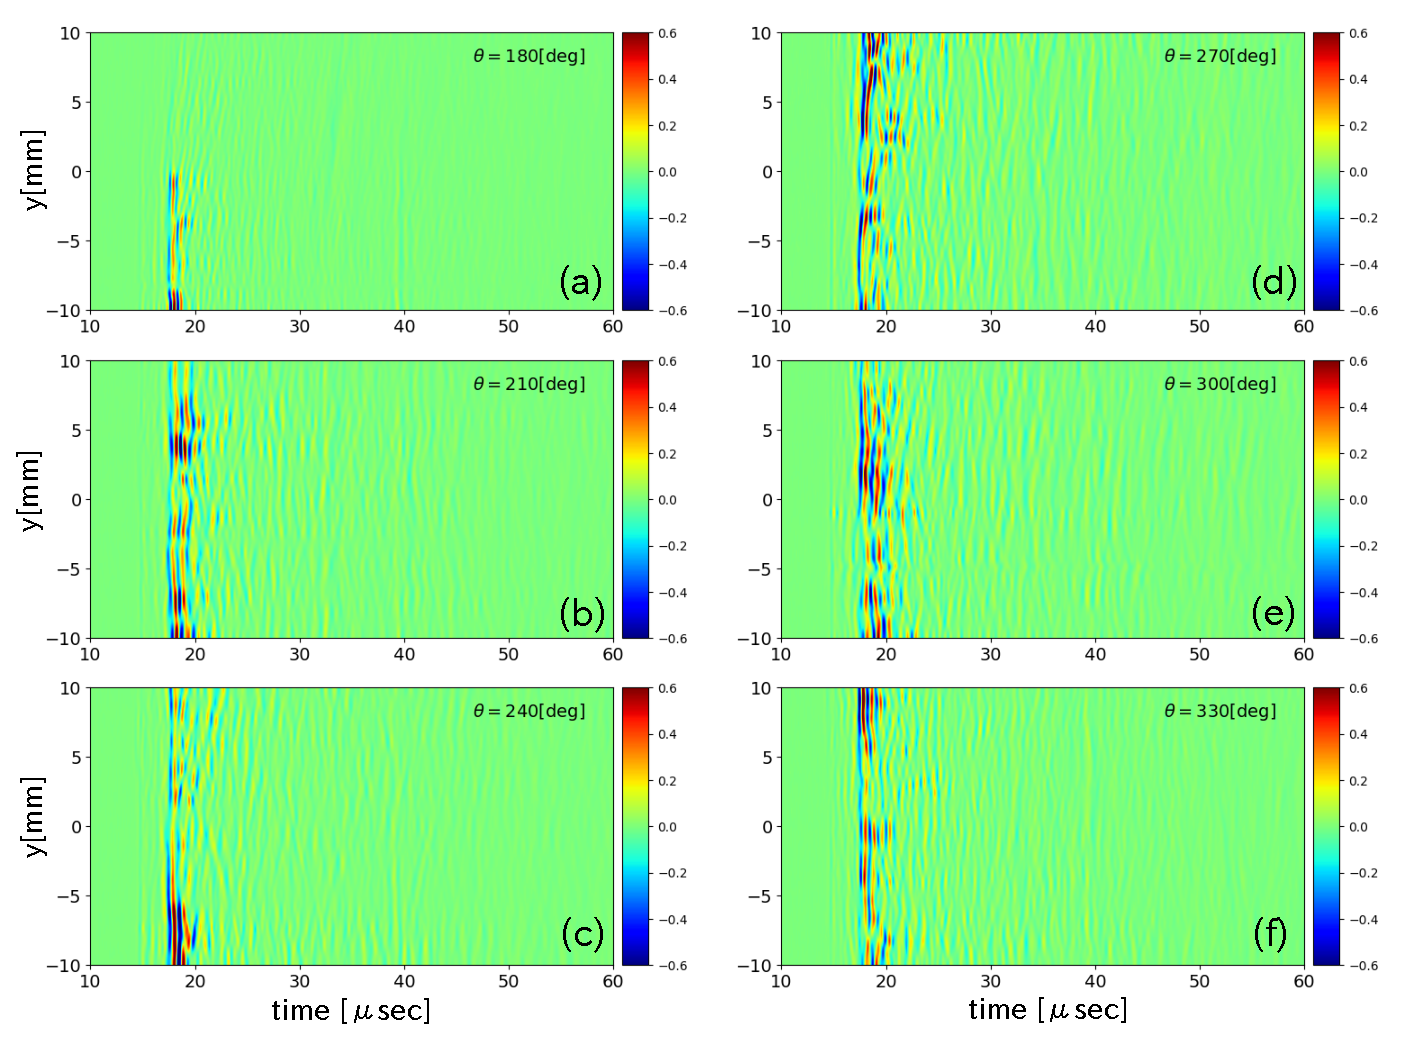
\includegraphics[width=1.0\linewidth]{Figs/fig5_3.eps} 
	\end{center}
	\caption{
		透過波波形の走時プロット(入射方向$\theta=180\sim 330^{\circ}$)
	} 
	\label{fig:fig5_3}
\end{figure}
%%%%%%%%%%%%%%%%%%%%%%%%%%%%%%%%%%%%%%%%%%%%%%%%%%%%%%%%%%%%%%%%%%%%%%
%%%%%%%%%%%%%%%%%%%%%%%%%%%%%%%%%%%%%%%%%%%%%%%%%%%%%%%%%%%%%%%%%%%%%%
\subsection{伝播速度の評価}
観測波形の初動成分を対象として伝播速度を評価するために、計測波形に時間軸上で
窓関数を作用させ、初動部近傍の大きな振幅を持つ波形部分を取り出す。
窓関数には、次式で与えられるButterworth関数を用いる。
\begin{equation}
	W(t;t_{1/2},m)=
	\left\{
		1+\left(\frac{t}{t_{1/2}}\right)^m
	\right\}^{-1}
	\label{eqn:Butterworth}
\end{equation}
Butterworth関数は、$m$が偶数のとき$t=0$について対称である。
その場合、$t_{1/2}$は振幅が半分となる時刻を、$m$は$t\rightarrow \pm \infty$
における減衰の速さを制御するパラメーターとして機能する。
ここで、$\cal R$上の位置$y$で観測される時間波形$a_{raw}(y,t)$とすれば、
Butterworth窓関数をかけて取り出された波形は
\begin{equation}
	a(y,t)=a_{raw}(y,t)W(t-t_b;t_{1/2},m)
\end{equation}
と表わされる。ここで、
\[
	t_b=18.2[\mu sec], \ \ t_{1/2}=2[\mu sec], \ \ m=6
\]
として観測波形に窓関数を作用させると、$\theta=0$[deg]では、図\ref{fig:6}の
ような結果が得られる。これを、図\ref{fig:fig5_2}-(a)を比べると、初動部分の
波形をほとんど変化させること無く、コーダ波が消去されていることが分かる。
次に、$a(y,t)$の時間に関するフーリエ変換を
\begin{equation}
	A(y, \omega)=\int a(y, t)e^{-i\omega t}dt=\left| A(\omega) \right|e^{i\phi}
	\label{eqn:def_FFT}
\end{equation}
を計算し、スペクトログラムとして表示すると、図\ref{fig:fig7}のようになる。
スペクトログラムからは、いずれの観測点位置における波形もおよそ3MHz程度までの
周波数成分が含まれており、入射波の持つ周波数成分を大きく損なうことなく、
岩石中を超音波が透過していることが分かる。
なお、図\ref{fig:fig6}に白の実線で示した時刻は、各観測点で得られた波形が
負の最大値を示す時刻を表している。一方、図\ref{fig:fig7}における白の実線は、
フーリエ振幅の最大値を与える周波数を示す。


岩石供試体中の弾性波の平均的な伝播挙動について調べるために、入射方向毎、すなわち測線毎に
平均波形を合成する。ここで、空間変数$y$に関する平均化作用素を
\begin{equation}
	\left< \cdot \right> := 
	\frac{1}{ \left| {\cal R} \right| }\int_{\cal R}\left( \cdot \right)dy
	\label{eqn:averaging}
\end{equation}
と表すことにすれば、波形データ${\cal D}$
\begin{equation}
	{\cal D}(\theta)=\left\{ a(y,t) \left| y\in {\cal R}, \, {\cal S}(\theta)\right.\right\}
	\label{eqn:}
\end{equation}
に対する平均波形は
\begin{equation}
	\left< a\right>(t)=
	\frac{1}{\left| {\cal R}\right|}\int_{\cal R}a(y,t)dy
	\label{eqn:def_mean_wv}
\end{equation}
で計算することができる。ただし、$\left| {\cal R }\right|$は、測線$\cal R$の長さ(20mm)を表す.
図\ref{fig:fig8}に、式(\ref{eqn:def_mean_wv})に従って計算した平均波形$\left<a \right>(t)$を
$\theta=0$[deg]の場合について、オレンジの実線で示す。この図には、ラインフォーカス探触子
のシュー先端部における自由振動波形$a^{ref}(t)$を参照波として青の実線で示している。
両者の振幅値は大きく異なることから、この図には二乗ノルムで正規化した結果を示している。
これらの波形の周波数スペクトルは、図\ref{fig:fig9}のようであり、透過波の平均波形は
参照波形と比べ2MHz以上の周波数成分が小さく、伝播の過程で相対的に高い周波成分が
多重散乱の結果コーダ波に転じている。

平均的な伝播速度の評価には、群速度$c_g$と,計測波形と参照波形の相互相関関数から評価した速度を
$c_{cor}$を用いる。ここでは、後者を"相互相関速度"と呼ぶことにする。
各々の定義は以下のようである。
\paragraph{群速度}
波形$v(t)$のフーリエ変換を
\begin{equation}
	V(\omega)=\int v(t)e^{-i\omega t} dt = \left| V(\omega) \right|e^{i\phi(\omega)}
	\label{eqn:phase}
\end{equation}
とし、その、アンラップされた位相角を$\phi(\omega)$とする。このとき、波形$v(t)$の
群遅延$t_g(\omega)$は
\begin{equation}
	t_g(\omega)=-\frac{d\phi}{d\omega}
	\label{eqn:def_gdelay}
\end{equation}
で与えられる.
図\ref{fig:fig11}は,位相角$\phi(\omega)$を平均波形$\left<a\right>(t)$と参照波形$a^{ref}(t)$
について実際に計算したものである。両者とも周波数に対して直線的に変化しており
線形位相遅れでよく近似できることが分かる。そこで、式(\ref{eqn:def_gdelay})の微分を
位相角を直線で最小2乗近似したときの直線の勾配として評価する。
そのため、$t_g$は周波数依存性はなくなり、一つの波形に対して一つの群遅延が与えられることになる。
このような方法で求めた、観測波形と参照波形の群遅延をそれぞれ$t_g, t_g^{ref}$とし、
観測波の透過距離を$L$とすれば、群速度$c_g$は
\begin{equation}
	c_g=\frac{L}{t_g-t_g^{ref}}
	\label{eqn:def_cg}
\end{equation}
で与えられる.位置$y$で得られた波形について計算した群速度を$c_g(y)$とすれば、その$y$に関する
平均$\left< c_g \right>$を考えることができる。また、平均波形$<a>(t)$についても群速度を
求めることができ、この意味での平均群速度を $\bar c_g$と表す。
$\bar c_g$と$\left< c_g \right>$とも、入射方向毎に求めることができるため、
入射方向への依存性を明示する際には、それぞれ、$\bar c_g(\theta), \left< c_g\right>(\theta)$
と書くことにする。
\paragraph{相互相関速度}
参照波形$a^{ref}(t)$と観測波形$a(t)$の相互相関関数を
\begin{equation}
	{\rm Cor}\left(a,a^{ref}\right)(t)=
	\frac{
	\int a(\tau)a^{ref}(\tau-t) d\tau
	}{
		\left\| a(t)\right\|
		\left\| a^{ref}(t)\right\|
	}
	\label{eqn:def_Cor}
\end{equation}
で定義する。Cor$(a,a^{ref}(t)$のピークを与える時刻$t_{f}$、すなわち
\begin{equation}
	t_{f}:={\rm argmax} \left\{
		-{\rm Cor}\left(a,a^{ref}\right)(t)
		\right\}
	\label{eqn:def_tof}
\end{equation}
を波動の到達時刻と考えれば,透過波の伝播速度(相互相関速度)は
\begin{equation}
	c_{cor}=\frac{L}{t_{f}}
	\label{eqn:}
\end{equation}
で求めることができる。このようにして決定した相互相関速度についても空間平均と、
平均波形に対するものを考えることができる。それぞれ、群速度の場合と同様、
$\bar c_{cor}(\theta), \left< c_{cor}\right>(\theta)$
と書くこととする。
図\ref{fig:fig11}は、式(\ref{eqn:def_Cor})によって計算した相互相関関数を
示したものである。横軸は時間$t$を、縦軸は波形観測位置$y$を表し、観測点毎に得られる
相互相関関数値をカラー表示している。
図中の白の実線は、相互相関関数の負のピーク位置$t_{f}$を示している。
%--------------------
\begin{figure}[h]
	\begin{center}
	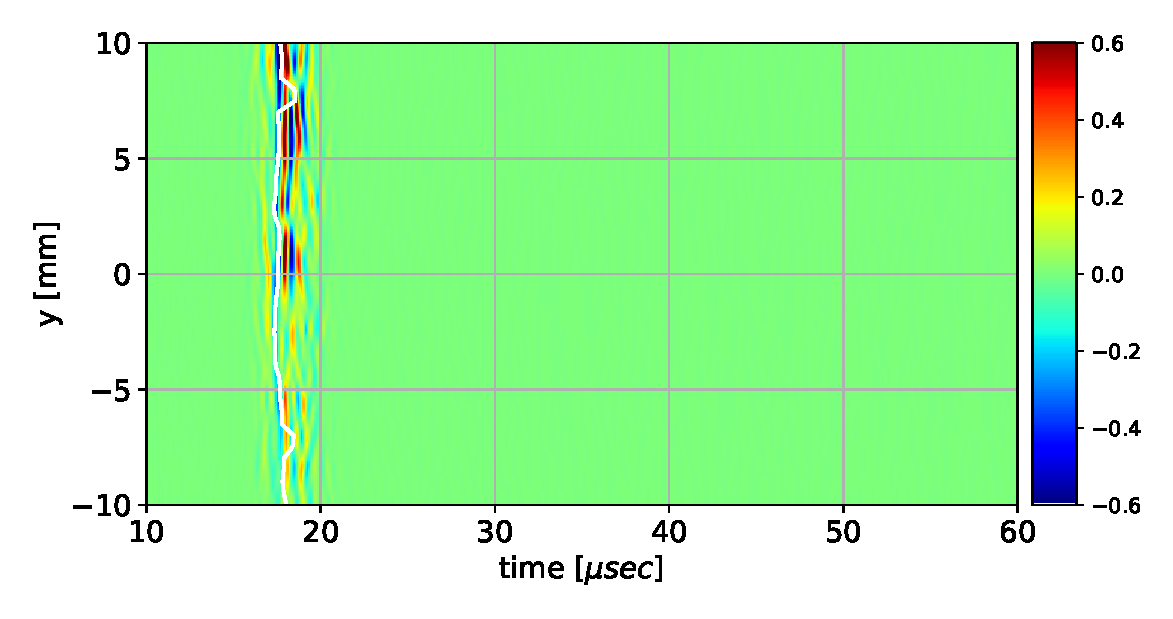
\includegraphics[width=0.7\linewidth]{Figs/fig6.eps} 
	\end{center}
	\caption{
		Butterworth窓関数で初動部分を取り出した結果の一例
		(入射方向$\theta=0^{\circ}$の場合)
	} 
	\label{fig:fig6}
\end{figure}
%--------------------
\begin{figure}[h]
	\begin{center}
	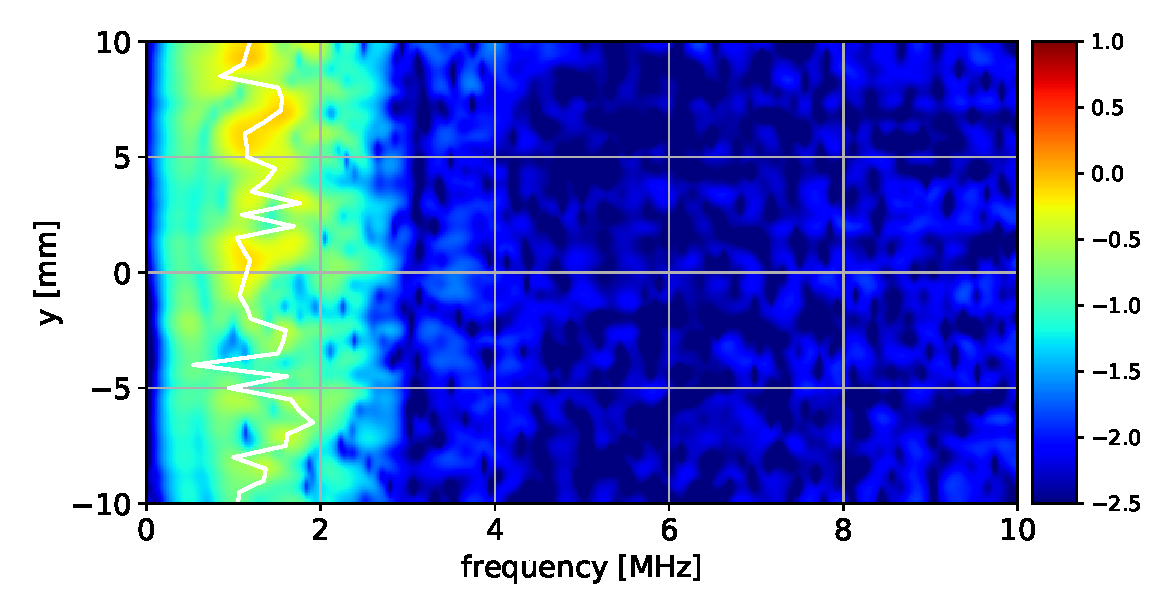
\includegraphics[width=0.7\linewidth]{Figs/fig7.eps} 
	\end{center}
	\caption{
		計測波形の初動部分に対する周波数スペクトログラム(入射方向$\theta=0^{\circ}$の場合).
	} 
	\label{fig:fig7}
\end{figure}
%--------------------
\begin{figure}[h]
	\begin{center}
	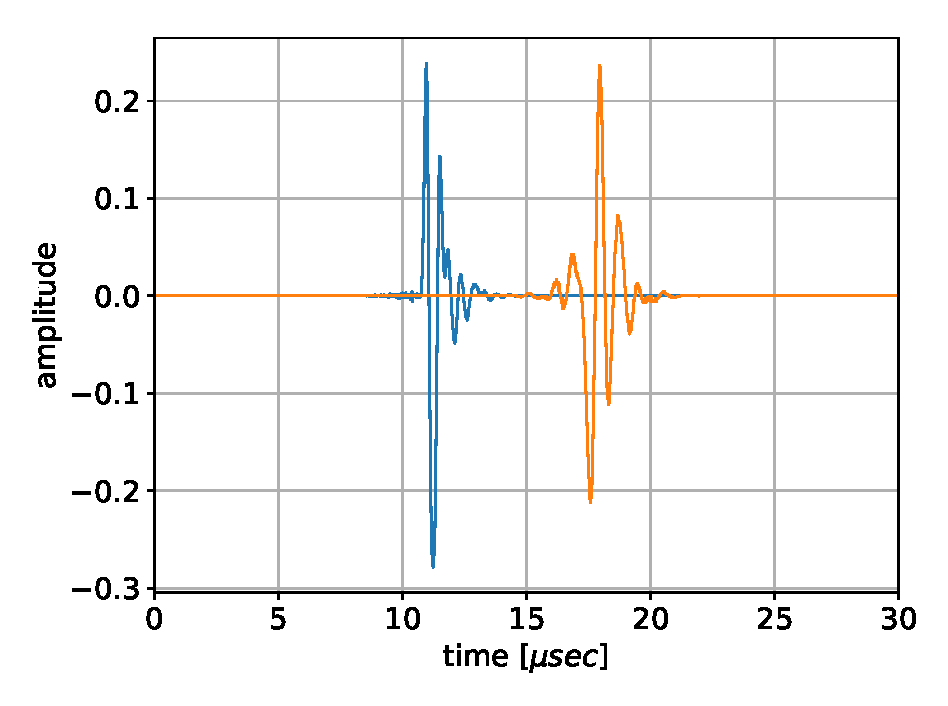
\includegraphics[width=0.6\linewidth]{Figs/fig8.eps} 
	\end{center}
	\caption{
		平均波形の時刻歴(オレンジの実線、入射方向$\theta=0^{\circ}$の場合).
		青はラインフォーカス探触子シュー先端部の自由振動波形に窓関数を
		作用させたものを参照波形として示す。
	} 
	\label{fig:fig8}
\end{figure}
%--------------------
\begin{figure}[h]
	\begin{center}
	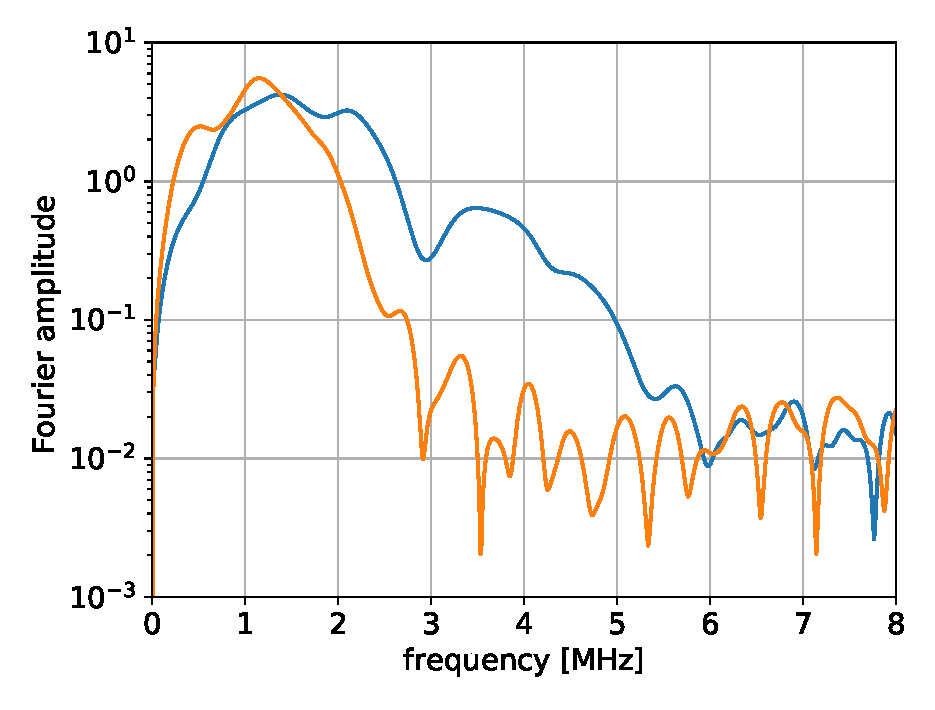
\includegraphics[width=0.6\linewidth]{Figs/fig9.eps} 
	\end{center}
	\caption{
		平均波形(オレンジ)と参照波形(青、シュー先端部の自由振動波形)の周波数スペクトル
		(入射方向$\theta=0^{\circ}の場合$).
	} 
	\label{fig:fig9}
\end{figure}
%--------------------
\begin{figure}[h]
	\begin{center}
	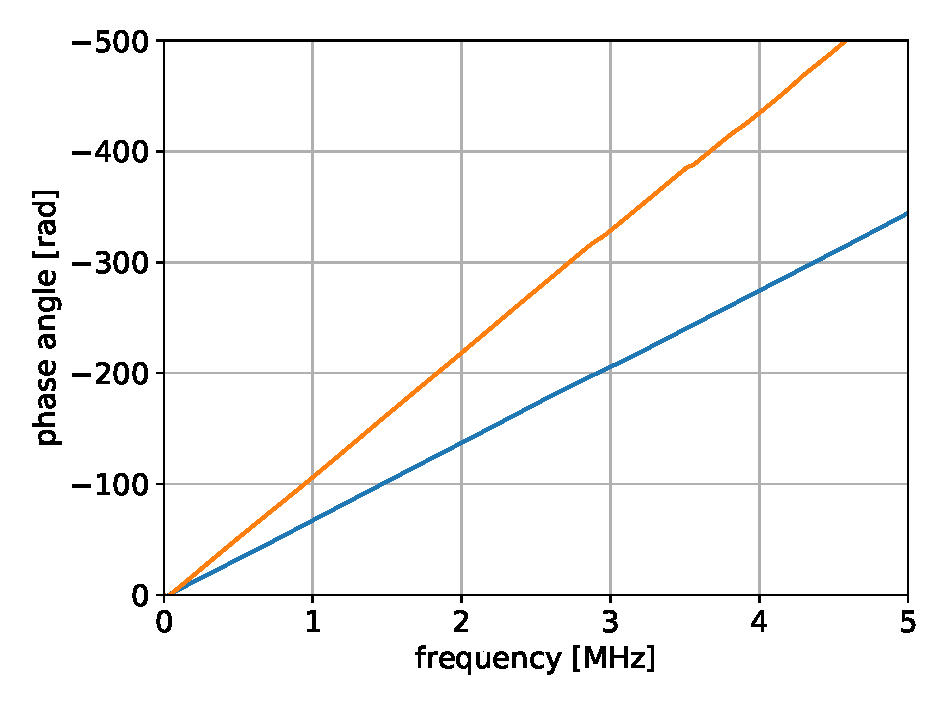
\includegraphics[width=0.7\linewidth]{Figs/fig10.eps} 
	\end{center}
	\caption{
		平均波形(オレンジ)と参照波形(青)の位相スペクトル(入射方向$\theta=0^{\circ}$の場合).
	} 
	\label{fig:fig10}
\end{figure}
%--------------------
\begin{figure}[h]
	\begin{center}
	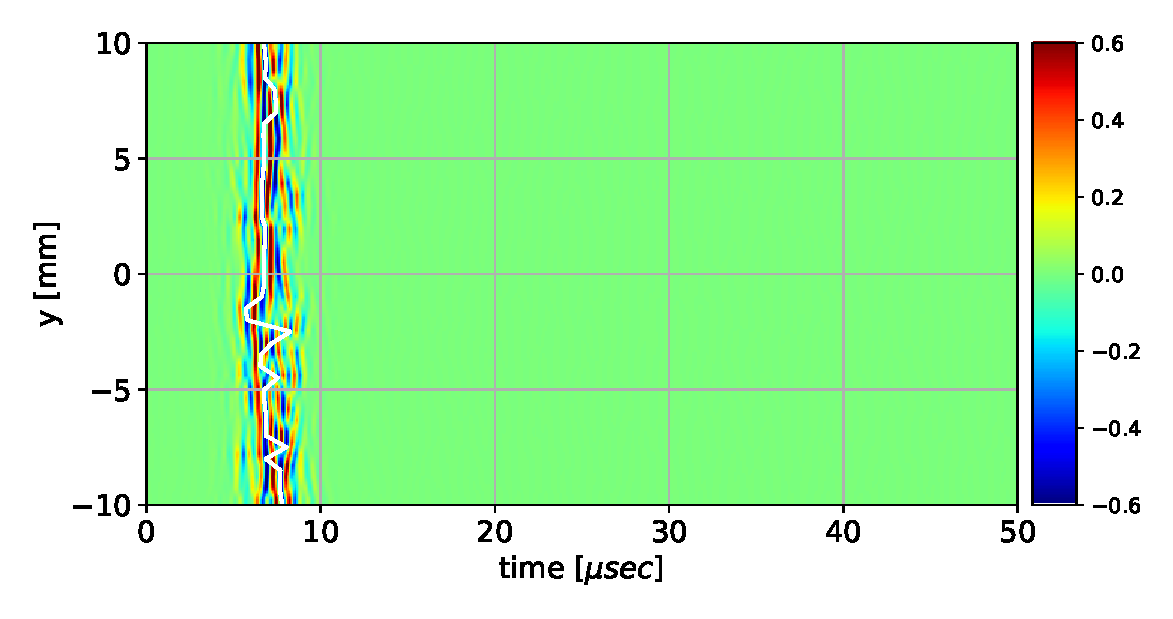
\includegraphics[width=0.7\linewidth]{Figs/fig11.eps} 
	\end{center}
	\caption{
		観測波形$a(y,t)$と参照波形$a^{ref}(t)$の時間に関する相互相関関数(入射方向$\theta=0^{\circ}$の場合).
	} 
	\label{fig:fig11}
\end{figure}
%--------------------

